\section{\label{sec:lattice}Lattice computation}

References: \cite{Hart2008,Hart2009,Cohen1993,CSE206A}

\subsection{Basis of lattice and unimodular matrix}

The choice of basis vectors is not unique for a given lattice.
A lattice spanned by basis vectors $( \bm{a}_{1}, \dots, \bm{a}_{n} )$ and a lattice spanned by
\begin{align}
  ( \bm{a}_{1}', \dots, \bm{a}_{n}' ) \coloneqq ( \bm{a}_{1}, \dots, \bm{a}_{n} ) \bm{P}
\end{align}
coincide if and only if $\bm{P}$ is a unimodular matrix, which is an integer matrix with $\det \bm{P} = \pm 1$\footnote{
  Let $L_{\bm{A}}$ be a lattice spanned by basis $\bm{A} = ( \bm{a}_{1}, \dots, \bm{a}_{n} )$.
  When $\bm{P}$ is unimodular, $L_{\bm{A}}$ contains $L_{\bm{AP}}$ because $\bm{P}$ is an integer matrix; $L_{\bm{AP}}$ contains $L_{\bm{A}}$ because the inverse of the unimodular matrix, $\bm{P}^{-1}$, is also an integer matrix; Thus, $L_{\bm{A}}$ and $L_{\bm{AP}}$ coincide.
  Conversely, when $L_{\bm{A}}$ and $L_{\bm{AP}}$ coincide, both $\bm{P}$ and $\bm{P}^{-1}$ should be integer matrices; Then, $\bm{P}$ is a unimodular matrix.
}.

% \subsubsection{Delaunay reduction}
%
% The Delaunay reduction\footnote{
%   Named after Boris Nikolayevich Delaunay or Delone.
% } is one of the lattice reduction algorithms to obtain a standardized basis.
% Given a basis $(\bm{b}_{1}, \dots, \bm{b}_{n})$, the Delaunay reduction updates the basis as follows:
% \begin{enumerate}
%   \item Consider a extended vector $\bm{b}_{n+1} \coloneqq -\sum_{i=1}^{n} \bm{b}_{i}$;
%   \item If $\bm{b}_{i} \cdot \bm{b}_{j}$ is positive for some $1 \leq i < j \leq n + 1$, update the basis as
%     \begin{equation}
%     \begin{aligned}
%       \bm{b}_{i}' &= -\bm{b}_{i} \\
%       \bm{b}_{j}' &= \bm{b}_{j} \\
%       \bm{b}_{k}' &= \bm{b}_{i} + \bm{b}_{k} \quad (k \neq i, j)
%     \end{aligned}
%     \end{equation}
%   \item Go back to the initial step until all products $\bm{b}_{i} \cdot \bm{b}_{j}$ are non-positive.
% \end{enumerate}
%
% until the sum
% \begin{align}
%   S = \sum_{i=1}^{n} \norm{\bm{b}_{i}}^{2}
% \end{align}
% cannot be decreased as follows:

\subsection{Sublattice, Hermite normal form, and their applications}

\subsubsection{Sublattices}

A \term{sublattice} is a subset of lattice $L$ obtained by removing some lattice points from $L$\footnote{
  In other fields than mathematics and crystallography, a substructure of a crystal structure is called a ``sublattice'', and a superstructure of a crystal structure is called a ``superlattice''.
}.
A set of basis vectors of the sublattice is identified with the transformation matrix $\bm{M}$ such that the original set of basis vectors $\bm{A}$ is transformed into a new set of basis vectors $\bm{AM}$.
Therefore, the sublattice $L_{\bm{AM}}$ is the set of lattice points expressed as
\begin{align}
  L_{\bm{AM}} = \set{ \bm{AMn} }{ \bm{n} \in \mathbb{Z}^{3} }.
\end{align}
We refer to the absolute value of the determinant of $\bm{M}$, $\det \bm{M}$, as the index of the sublattice $L_{\bm{AM}}$.
The index is identical to the number of lattice points in the sublattice $L_{\bm{AM}}$.

\subsubsection{Hermite normal form}

Let $\bm{U}$ be a three-dimensional square unimodular matrix.
Two transformation matrices $\bm{M}$ and $\bm{MU}$ give the same sublattice, $L_{\bm{AM}} = L_{\bm{AMU}}$.
Among the equivalent transformation matrices, their representative can be chosen by the \term{Hermite normal form} (HNF).
A transformation matrix $\mathbf{M}$ can be converted to a unique lower-triangular integer matrix, HNF, by multiplying a unimodular matrix $\mathbf{U'}$ from the right with
\begin{align}
    \label{eq:HNF}
    \bm{MU'} =
    \left(
    \begin{array}{ccc}
         a & 0 & 0 \\
         b & c & 0 \\
         d & e & f
    \end{array}
    \right),
\end{align}
where $a > 0$, $0 \leq b < c$, $0 \leq d < f$, and $0 \leq e < f$.
% More mathematically it results from the fact $\mathbf{U}^{-1}$ is also a unimodular matrix.
% HNF
The requirement that diagonal elements $a$, $c$, and $f$ are all positive eliminates equivalent basis vectors obtained by inversion.
Also, the addition of a basis vector to another one or the subtraction of a basis vector from another one does not change the lattice itself.
Thus, we can choose remainders of $f$ as $d$ and $e$, and a remainder of $c$ as $b$.

Let us generalize HNFs to $m \times n$ integer matrix, $\bm{M}$.
It has a (column-style) Hermite normal form $\bm{H}$ if there exists a unimodular matrices $\bm{R} \in \mathbb{Z}^{n \times n}$ such that $\bm{H}=\bm{MR}$ satisfied the following conditions
\begin{enumerate}
    \item $H_{ij} \geq 0 \quad (1 \leq i \leq m, 1 \leq j \leq n)$
    \item $H_{ij} = 0 \quad (i < j , j > r)$
    \item $H_{ij} < H_{ii} \quad (i > j, 1 \leq i \leq r)$
    \item $r = \mathrm{rank} \bm{M}$
\end{enumerate}

If $\mathbf{M}$ is full rank, the Hermite normal form $\bm{H}$ is uniquely determined.

\subsubsection{\label{sec:hnf-computation}Procedure to compute HNF}

We can obtain the HNF of an integer matrix by applying the following elementary operations consecutively,
\begin{itemize}
  \item (Column swap) swapping the $i$th and $j (\neq i)$th columns,
  \item (Column sign change) multiplying the $i$th column by $-1$,
  \item (Column addition) adding $k \in \mathbb{Z}$ multiples of the $j$th column to the $i$th column.
\end{itemize}
The coefficient $k$ in the column addition should be an integer because the matrix should be an integer matrix after applying the operation.

For a given integer matrix $\bm{M} \in \mathbb{Z}^{m \times n}$, we process from the first to the $m$th rows.
When we process the $s$th row, we select the $i^{\ast}$th column such that $i^{\ast} = \underset{i = s, \dots, n, M_{si} \neq 0}{\arg\min} |M_{si}|$;
we add the $i^{\ast}$ column to the other $j$th columns so that $|M_{sj}|$ decreases;
We continue this process until all $|M_{sj}|$ cannot decrease.

Here is an example to compute HNF for a two-dimensional matrix.
\begin{align*}
  \begin{pmatrix}
    20 & -6 \\
    -2 & 1 \\
  \end{pmatrix}
  &\overset{\mbox{swap}}{\longrightarrow}
  \begin{pmatrix}
    -6 & 20 \\
    1 & -2 \\
  \end{pmatrix}
  \overset{\mbox{sign}}{\longrightarrow}
  \begin{pmatrix}
    6 & 20 \\
    -1 & -2 \\
  \end{pmatrix}
  \overset{\mbox{add}}{\longrightarrow}
  \begin{pmatrix}
    6 & 2 \\
    -1 & 1 \\
  \end{pmatrix}
  \overset{\mbox{swap}}{\longrightarrow}
  \begin{pmatrix}
    2 & 6 \\
    1 & -1 \\
  \end{pmatrix} \\
  &\overset{\mbox{add}}{\longrightarrow}
  \begin{pmatrix}
    2 & 0 \\
    1 & -4 \\
  \end{pmatrix}
  \overset{\mbox{sign}}{\longrightarrow}
  \begin{pmatrix}
    2 & 0 \\
    1 & 4 \\
  \end{pmatrix}
\end{align*}

\subsubsection{Union of lattices}

We introduce the procedure to take the union of lattices as an application of HNF.
Given dependent vectors $\bm{b}_{1}, \dots, \bm{b}_{k} \in \mathbb{Z}^{n}$, we find the smallest basis $\bm{b}_{1}', \dots, \bm{b}_{r}' \, (r \leq k)$ with
\begin{align*}
  L_{\left( \bm{b}_{1}, \dots, \bm{b}_{k} \right)} = L_{ \left( \bm{b}_{1}', \dots, \bm{b}_{r}' \right) }.
\end{align*}
It is easily solved by computing the HNF of $\left( \bm{b}_{1}, \dots, \bm{b}_{k} \right)$ and taking nonzero columns.

For example, consider the union of a $2 \times 2 \times 2$ sublattice and a body-centering translation.
The HNF of the basis vectors is
\begin{align*}
  \begin{pmatrix}
    2 & 0 & 0 & 1 \\
    0 & 2 & 0 & 1 \\
    0 & 0 & 2 & 1 \\
  \end{pmatrix}
  \longrightarrow
  \begin{pmatrix}
    1 & 0 & 0 & 0 \\
    1 & 2 & 0 & 0 \\
    1 & 0 & 2 & 0 \\
  \end{pmatrix}.
\end{align*}
Thus, the union of lattices is spanned by $\begin{pmatrix} 1 \\ 1 \\ 1 \end{pmatrix}$, $\begin{pmatrix} 0 \\ 2 \\ 0 \end{pmatrix}$, and $\begin{pmatrix} 0 \\ 0 \\ 2 \end{pmatrix}$.

\subsubsection{\label{sec:integer-linear-system}Integer linear system}

For given $\bm{A} \in \mathbb{Z}^{m \times n}$ and $\bm{b} \in \mathbb{Z}^{m}$, consider to solve integer linear system $\bm{Ax} = \bm{b}$ in $\bm{x} \in \mathbb{Z}^{n}$.
Let the Hermite normal form of $\bm{A}$ be $\bm{H} = \bm{AR}$, where $\bm{R}$ is unimodular and $\bm{H}$ is lower triangular.
The given linear system is
\begin{align}
  \begin{pmatrix}
    H_{11} &        & \bm{O} & \vdots     \\
    \vdots & \ddots &        & \bm{0} \\
    H_{r1} & \ldots & H_{rr} & \vdots     \\
    \ldots & \bm{0} & \ldots & \bm{O} \\
  \end{pmatrix}
  \bm{y} = \bm{b}
\end{align}
where $\mathbf{y} \coloneqq \bm{R}^{-1}\bm{x}$.
A special solution, $\bm{x}_{\mathrm{special}} = \bm{R}\bm{y}_{\mathrm{special}}$, is determined by Gaussian elimination if exists.
A general solution for $\bm{Hy}=\bm{0}$ is given by
\begin{align}
  \bm{y} = \begin{pmatrix} 0 \\ \vdots \\ 0 \\ n_{r+1} \\ \vdots \\ n_{m} \end{pmatrix}
        \quad (\forall n_{r+1},\dots, n_{m} \in \mathbb{Z}).
\end{align}

\subsection{Smith normal form and its applications}

\subsubsection{Distinct lattice points in sublattice}

When we consider the translational symmetry of a sublattice $L_{\bm{AM}}$, two lattice points, $\bm{m}$ and $\bm{m}$, are equivalent if the displacement between the two lattice points is a translation of $L_{\bm{AM}}$, that is,
\begin{align}
  \label{eq:equiv-lattice-points}
  \bm{m} - \bm{m}' \in \bm{M}\mathbb{Z}^{3}.
\end{align}

The \term{Smith normal form} (SNF) of the transformation matrix $\mathbf{M}$ is useful to concretely write down Eq.~\eqref{eq:equiv-lattice-points} \cite{PhysRevB.77.224115}.
The SNF is one of the decompositions of an integer matrix $\mathbf{M}$ as
\begin{align}
  \label{eq:SNF}
  \bm{D} = \bm{PMQ},
\end{align}
where $\bm{P}$ and $\bm{Q}$ are unimodular matrices, and $\mathbf{D}$ is a diagonal integer matrix,
\begin{align}
  \bm{D} =
      \begin{pmatrix}
          D_{11} & 0 & 0 \\
          0 & D_{22} & 0 \\
          0 & 0 & D_{33}
      \end{pmatrix}.
\end{align}
Here $D_{11}$ is a divisor of $D_{22}$, and $D_{22}$ is a divisor of $D_{33}$.
We can rewrite Eq.~\eqref{eq:equiv-lattice-points} with Eq.~\eqref{eq:SNF} as
\begin{align}
  \label{eq:equiv-represents}
  \bm{m} - \bm{m}' \in \bm{M} \mathbb{Z}^{3}
    &\Leftrightarrow \bm{m} - \bm{m}' \in \bm{P}^{-1} \bm{D} \mathbb{Z}^{3} \nonumber \\
    &\Leftrightarrow \bm{Pm} - \bm{Pm}' \in \bm{D} \mathbb{Z}^{3} \nonumber \\
    &\Leftrightarrow [\bm{Pm}]_{\bm{D}} = [\bm{Pm}']_{\bm{D}},
\end{align}
where $[\cdot]_{\bm{D}}$ indicates to take modulus for the $i$th row by $D_{ii}$.
We mention that the range of $[\cdot]_{\mathbf{S}}$ is $\mathbb{Z}_{D_{11}} \times \mathbb{Z}_{D_{22}} \times \mathbb{Z}_{D_{33}}$ because a value of the $i$th row is a remainder by $D_{ii}$.

For example, Fig.~\ref{fig:hnf_supercell} shows a sublattice of the square two-dimensional lattice with a transformation matrix
\begin{align*}
  \bm{M} =
  \begin{pmatrix}
    2 & 0 \\
    1 & 4 \\
  \end{pmatrix}.
\end{align*}
The SNF of the transformation matrix is
\begin{align*}
  \begin{pmatrix} 1 & 0 \\ 0 & 8 \end{pmatrix}
  =
  \begin{pmatrix} 0 & 1 \\ -1 & 2 \end{pmatrix}
  \bm{M}
  \begin{pmatrix} 1 & -4 \\ 0 & 1 \end{pmatrix}.
\end{align*}

\begin{figure}[htb]
  \centering
  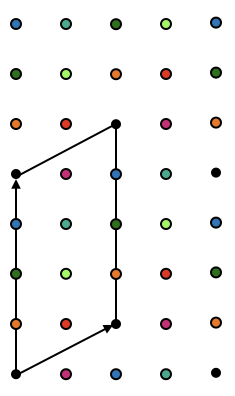
\includegraphics[width=0.3\textwidth]{figure/fig_supercell.png}
  \caption{
    Lattice points in a sublattice.
    The distinct lattice points are labeled with different colors.
  }
  \label{fig:hnf_supercell}
\end{figure}



\subsubsection{Smith normal form}

Let us generalize SNFs to $m \times n$ integer matrix $\bm{M}$.
There exist some unimodular matrices $\bm{P} \in \mathbb{Z}^{m \times m}$ and $\bm{Q} \in \mathbb{Z}^{n \times n}$ such that

\begin{align}
    \bm{D}
    \coloneqq
    \bm{PMQ}
    =
    \begin{pmatrix}
        d_{1}  &        & \bm{O} & \bm{0} \\
               & \ddots &        & \vdots \\
        \bm{O} &        & d_{r}  & \bm{0} \\
        \bm{0} & \cdots & \bm{0} & \bm{O}
    \end{pmatrix},
\end{align}
where $d_{i}$ is positive integer and $d_{i+1}$ devides $d_{i}$.
Then $\bm{D}$ is called Smith normal form.

\subsubsection{Procedure to compute SNF}

The SNF can be obtained by the elementary operations in Sec.~\ref{sec:hnf-computation} for both column-wise and row-wise.
After we process the $s$th row and column, the matrix looks
\begin{align*}
  \left(
    \begin{array}{ccc|c}
      d_{1} &        & \bm{O} &        \\
             & \ddots &        & \bm{O} \\
      \bm{O} &        & d_{s}  &        \\ \hline
             & \bm{O} &        & \ast   \\
    \end{array}
  \right)
\end{align*}
and the remained submatrix $\ast$ should be multiples of $d_{s}$.

Here is an example to compute HNF for a three-dimensional matrix.
\begin{align*}
  \begin{pmatrix}        2 & 4 & 4 \\        -6 & 6 & 12 \\        10 & -4 & -16 \\    \end{pmatrix}
  &\to    \begin{pmatrix}        2 & 0 & 0 \\        -6 & 18 & 24 \\        10 & -24 & -36 \\    \end{pmatrix}
  \to    \begin{pmatrix}        2 & 0 & 0 \\        0 & 18 & 24 \\        0 & -24 & -36 \\    \end{pmatrix}    \\
  &\to    \begin{pmatrix}        2 & 0 & 0 \\        0 & 18 & 6 \\        0 & -24 & -12 \\     \end{pmatrix}
  \to    \begin{pmatrix}        2 & 0 & 0 \\        0 & 18 & 6 \\        0 & 12 & 0 \\    \end{pmatrix}    \\
  &\to    \begin{pmatrix}        2 & 0 & 0 \\        0 & 6 & 18 \\        0 & 0 & 12 \\    \end{pmatrix}
  \to    \begin{pmatrix}        2 & 0 & 0 \\        0 & 6 & 0 \\        0 & 0 & 12 \\    \end{pmatrix}
\end{align*}

\subsubsection{Frobenius congruent}

For given $\bm{A} \in \mathbb{Z}^{m \times n}$ and $\bm{b} \in \mathbb{Z}^{m}$, consider to solve Frobenius congruent $\bm{Ax} \equiv \bm{b} \, (\mathrm{mod}\, \mathbb{R}/\mathbb{Z})$ for $\bm{x} \in \mathbb{R}^{n}$.
Let SNF of $\bm{A}$ be $\bm{D} = \bm{PAQ}$, where $\bm{P}$ and $\bm{Q}$ are unimodular matrices.
\begin{align}
  \bm{PAx} &= \bm{Pb} + \mathbb{Z}^{n} \\
  \bm{Dy}  &= \bm{v} + \mathbb{Z}^{n} \quad \mbox{where}\, \bm{y}:= \bm{Q}^{-1} \bm{x},\, \bm{v}:= \bm{Pb} \\
  \bm{y}
    &= \begin{pmatrix} \frac{v_{1}}{D_{11}} \\ \vdots \\ \frac{v_{r}}{D_{rr}} \\ 0 \\ \vdots \\ 0 \end{pmatrix}
        + \begin{pmatrix} \frac{1}{D_{11}} n_{1} \\ \vdots \\ \frac{1}{D_{rr}} n_{r} \\ 0 \\ \vdots \\ 0 \end{pmatrix}
        + \begin{pmatrix} 0 \\ \vdots \\ 0 \\ a_{r+1} \\ \vdots \\ a_{m} \end{pmatrix}
        \quad (\forall n_{1}, \dots, n_{r} \in \mathbb{Z}, \forall a_{r+1}, \dots, a_{m} \in \mathbb{R})
\end{align}
